\chapter{Methodology}

\section{Introduction}
VoteGuard Pro follows a security-first and accessibility-constrained methodology. The method combines modular software engineering, threat-informed design, and prototype validation.

The selected approach was chosen because it allows independent verification of critical layers (UI, storage, audit, and optional chain anchoring) while supporting rapid iteration in academic constraints.

\section{System Architecture}
The architecture follows clean-separation principles:
The core layer contains the domain models, ports, use cases, and the state machine. The adapter layer provides the encrypted storage adapter, the audit log adapter, the chain simulation path, and the device adapters. The UI layer handles Aadhaar entry, biometric capture, and the voting screen workflow, while the optional ML layer is used only for overlays and anomaly hints that improve operator observability.

Data flow:
The flow starts by capturing voter identifiers and initializing the voting session. It then performs biometric capture or face detection and continues the guided flow until the candidate selection is confirmed. After confirmation, the ballot payload is encrypted and appended to the hash-chained ledger, and the audit event is recorded while the optional chain-anchoring metadata is prepared.

\section{Algorithm}
Key algorithms and controls used:
The encrypted append algorithm encrypts the vote payload via Fernet, appends it as the next sequence element, and updates the chain hash. The cast-registry guard creates a salted identifier hash and rejects duplicate cast attempts. The ledger verification algorithm traverses the records to validate sequence continuity and previous-hash integrity. UI state progression remains deterministic so that screens advance without overlapping dialogs or race conditions.

Representative pseudocode:
\begin{verbatim}
Input: voter_id, candidate
if cast_registry.contains(hash_salt(voter_id)):
	reject_vote("duplicate attempt")
else:
	payload = encrypt({candidate, timestamp, station_id})
	record = append_hash_chain(payload)
	audit_log.append("vote_cast", record.hash)
	cast_registry.add(hash_salt(voter_id))
	confirm_success()
\end{verbatim}

\begin{figure}[htbp]
\centering
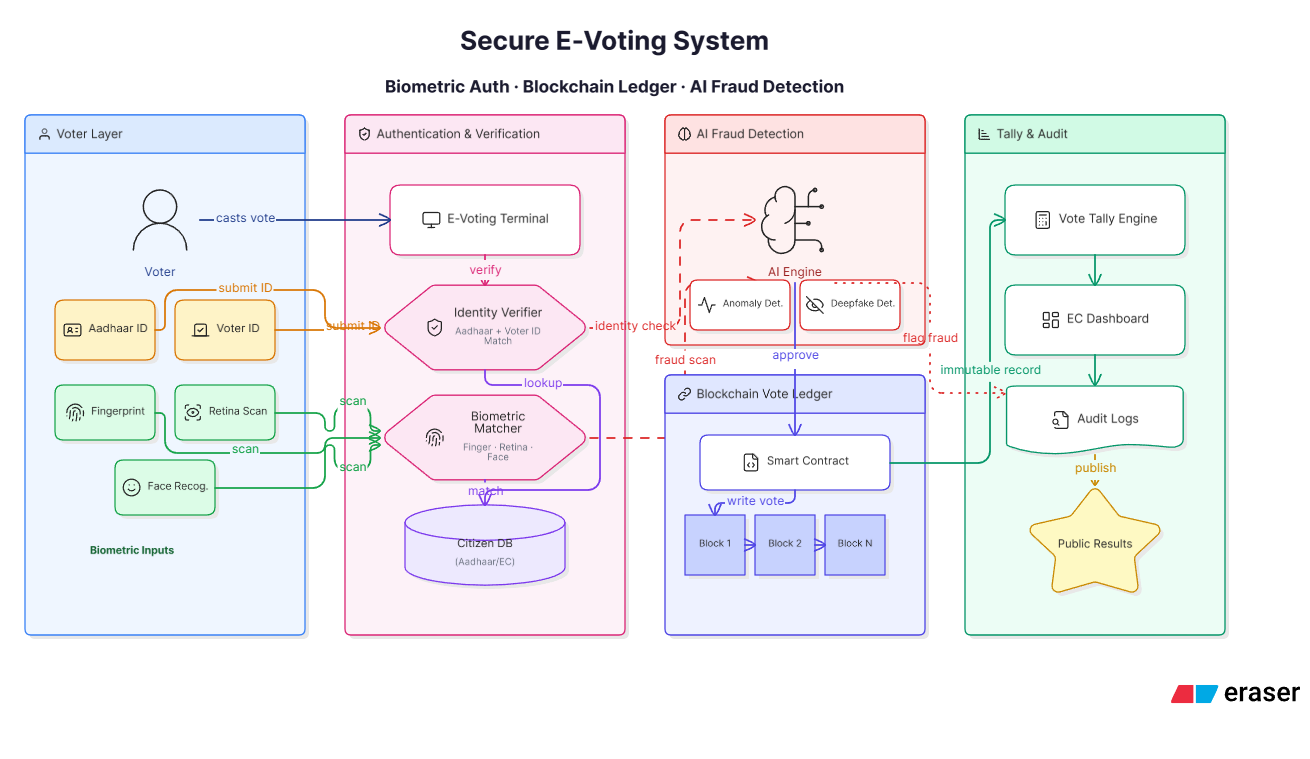
\includegraphics[width=0.9\textwidth]{assets/architecture.png}
\caption{High-Level System Architecture}
\figurelegend{Shows UI layer, core use-cases, encrypted ballot ledger, audit chain, and optional blockchain anchor path. Preconditions: voting session initialized, candidate list available, device stack active. Main flow: identifier entry → biometric capture → vote cast → encrypted storage. Postconditions: vote recorded, cast-registry updated, audit event persisted.}
\end{figure}
\subsection{Detailed Architecture Layers}

The system is organized in six layered tiers following clean architecture principles:

The presentation layer includes the Voter UI, Election Officer Dashboard, System Auditor Console, and REST API endpoints. The application layer contains the Session Manager, Vote Casting Orchestrator, Enrollment Validator, Verification Engine, and Tally Calculator. The domain layer holds the Voter Entity, Ballot Entity, Cast Registry, Cryptography Service, and State Machine. Dependency inversion is achieved through the IStorage, IAudit, IChainAnchor, and IDevice interfaces. The adapter layer is implemented through the StorageHashChainAdapter, AuditLogHashChainAdapter, ChainAnchorServiceAdapter, and DeviceMockAdapter, while the infrastructure layer includes the Encrypted File Store, Audit Records, Biometric Scanner, Card Reader, Printer, Blockchain Service, and Remote Verification.

\begin{figure}[htbp]
\centering
\fbox{\parbox[c][8cm][c]{0.95\textwidth}{Complete system architecture diagram with all six layers, component interactions, and data flows. See PlantUML file: \texttt{voteguard\_complete\_architecture.puml} or XML GraphML: \texttt{voteguard\_complete\_architecture.xml} in assets folder for detailed visualization.}}
\caption{Complete System Architecture - All Layers and Data Flows}
\figurelegend{Comprehensive architecture showing Presentation Layer invocations flowing to Application Layer use cases, which orchestrate Domain Layer entities and use Port Interfaces; Adapter Layer implements ports and interfaces with Infrastructure Layer components. All external access is routed through adapters to enforce clean architecture boundaries.}
\end{figure}
\clearpage
